
\chapter{Generation}

\section {Terrain}

\subsection{World Map}

The terrain is generated by first establishing a world map at course resolution, then selecting from a series of different landscape generators based on general elevation.
The world map uses a single distorted brownian layer with a box ramp to force oceans at all borders.

The base elevations are scaled for a theoretical maximum of 1000 feet and minimum of -750ft.
However, the individual landscape generators may produce values above or below these amounts.

\subsection{Regions}

For rendering the terrain values need to be generated at 1 foot postings.
We also need color values to shade the ground, and a forestation value to determine how to place trees.

Cubic interpolation is used to calculate a baseline elevation at each of these postings.
This elevation is then used to pick a particular generator to generate the final elevation value.
The individual generators are called regions in this system.
The baseline elevation is also used by the region generators to determine how to transition to neighbor regions.

Because the values generated for the world map are sparse (one posting every 1024 feet) it inherently lacks high frequency noise.
This makes it useful for generating features such as cliffs at the intersection between different elevations, because isolines adhere to the grid structure.
In general the use of a low resolution, low frequency baseline map helps keep individual regions separate without having areas that swap between multiple region types unrealistically.

\editor{Figure here showing isolines of the map}

The region types used by the engine are: Oceans, Beaches, Fields, Forests, Hills, Mountains, and Snowpeaks.

While each region generator is individually responsible for generating elevation values, some noise sources are shared between the different regions so that smooth transitions can be generated.
As an example, consider the following odd grouping of region types.

\subsubsection{Oceans, Fields, Forests}

The oceans, fields, and forests generators all simply add some high-frequency noise and coloring to the baseline elevation.
This generates small sandy hills below water for Oceans, small grassy hills for Fields, and tree-covered hills for Forests.

\subsubsection{Beaches}

Beaches serve as a transition between oceans and fields.
Beaches may contain a cliff partway between the shoreline and the transition to the field region.

This cliff is generated by applying a vertical offset to any baseline value above a certain threshold.
The offset is applied gradually over a small area so that the cliffs are not completely abrupt, but have a horizontal dimension of a few feet.
As the baseline elevation approaches the transition to Fields, the offset is tapered off to give cliffs some additional prominence.
See Figure~\ref{fig:beach_cliffs}.

The exact size, shape, and shoreline distance of the cliffs are influenced by additional noise values.

\begin{figure}
  \centering
    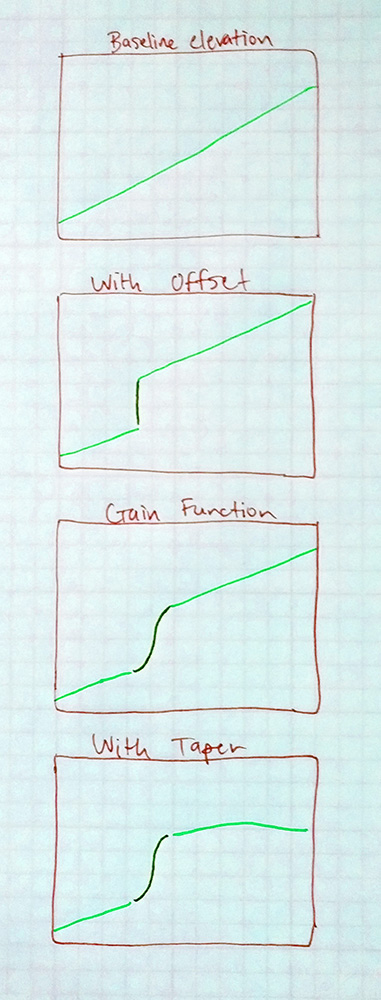
\includegraphics[width=0.5\textwidth]{figures/beach_cliffs}
  \caption{Beach cliff generation \editor{Temporarily hand-drawn}}
  \label{fig:beach_cliffs}
\end{figure}

\subsubsection{Hills and Mountains}
